\section{Flip-Flop tipo D con \textit{reset} síncrono \label{sec:s2}}

\begin{center}
	\begin{minipage}{12cm}
		\begin{tcolorbox}[title=Actividad 2]
			Codificar un flip-flop tipo D con \textit{reset} síncrono. Compilar y simular. Usar el visor RTL para observar como se implementa el circuito y mencionar diferencias con el circuito del inciso 1. Configurar en la tarjeta DE2-115, asignar interruptores y un LED.
		\end{tcolorbox}	
	\end{minipage}
\end{center}

La visualización RTL del flip flop tipo D con \textit{reset} síncrono en Verilog se muestra en la \autoref{fig:ff_d_syn_rtl}. En el visor se observa que la señal RST se conecta como señal de control de un multiplexor, cuya salida esta conectada a la terminal D del flip flop. Si el valor de RST es 0, entonces la salida adquiere el valor de la señal D, pero si el valor es 1, la salida será 0 (Este valor sería la representación del estado de restablecimiento). Las señales restantes se conectan a los pines correspondientes del modulo (CLK y Q).

Las simulaciones para el código en Verilog se visualizan en la \autoref{fig:ff_d_syn_wave}. Se observa que la salida Q adquiere el valor de la entrada D unicamente cuando en la señal de reloj (CLK) hay un flanco de subida. La limpieza en el flip flop se da de manera síncrona con el pin RST, ya que unicamente cuando CLK tiene un flanco de subida, el \textit{reset} ajustará el valor de la salida a 0.

En los Anexos se localiza la descripción del flip flop tipo D con \textit{reset} síncrono. Se utilizó una lista sensible para el flanco de subida de la señal de reloj. Dentro de esta estructura se empleó la sentencia \textit{if} para comparar el valor de RST: 
\begin{itemize}
	\item Si es 1, se restablece el valor de la salida a 0. 
	\item Si es 0, la salida adquiere el valor de D.
\end{itemize}

En la \autoref{fig:asyn_vs_syn_wave} se observa la comparativa de simulaciones del flip flop con \textit{reset} síncrono y asíncrono, viendo que el primero restablece el valor de la salida Q hasta que CLK tiene un flanco de subida, en cambio, el segundo hace el restablecimiento independientemente de la señal de reloj. Igualmente, se diferencian ambas implementaciones en las conexiones que se tienen en el RTL y en la descripción de cada modulo.

\begin{figure}[ht]
	\centering
	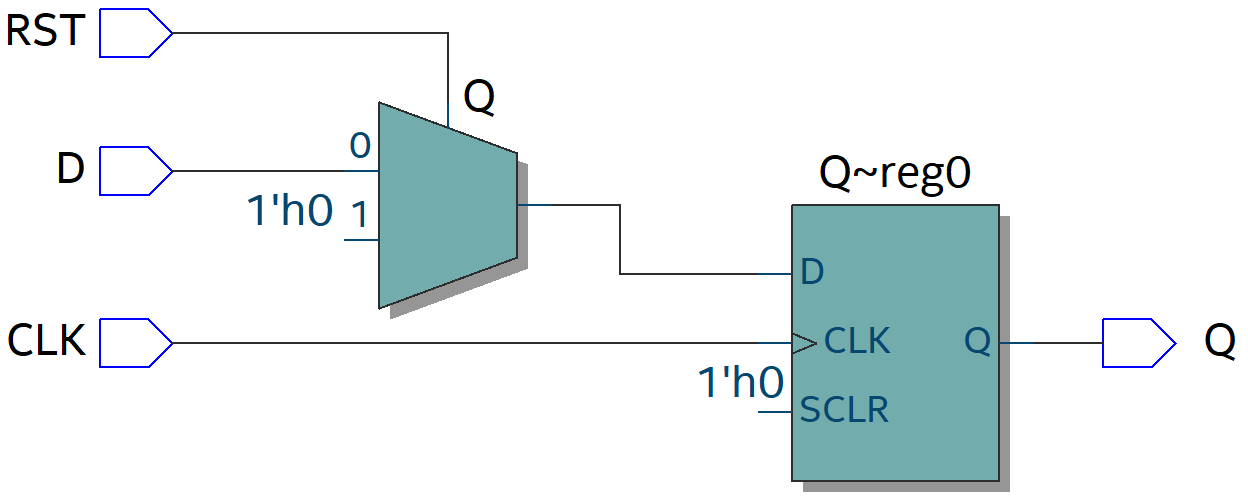
\includegraphics[scale=0.5]{FF_D_Syn_RST_RTL.png}
	\caption{Diagrama RTL del flip flop tipo D con \textit{reset} síncrono. \label{fig:ff_d_syn_rtl}}
\end{figure}

\begin{figure}[ht]
	\centering
	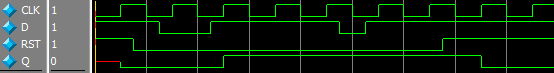
\includegraphics[scale=1.2]{FF_D_Syn_RST_Wave.png}
	\caption{Simulación del flip flop tipo D con \textit{reset} síncrono en el visor de formas de onda de ModelSim. 
	\label{fig:ff_d_syn_wave}}
\end{figure}

\begin{figure}[ht]
	\centering
	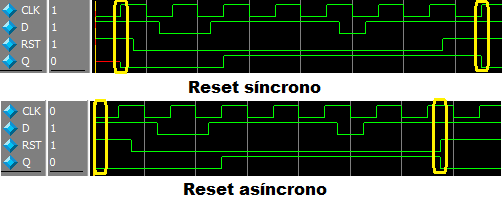
\includegraphics[scale=1.3]{Asyn_vs_Syn_RST.png}
	\caption{Comparativa del flip flop tipo D con \textit{reset} síncrono y asíncrono en el visor de formas de onda de ModelSim. Se observa que las señales de \textit{reset} son las mismas pero la ejecución de esta operación varía en cada caso.
	\label{fig:asyn_vs_syn_wave}}
\end{figure}